Šiais laikais labai daug yra kalbama apie dirbtinį intelektą, robotus, kurie jau dabar yra naudojami padedant žmonėm atlikti kasdienius darbus ir netgi robotai keičia žmones gamyklose atliekant specifinius darbus.

Šiuolaikinėje visuomėneje, turbūt nei vienas negali įsivaizduoti gyvenimo be telefono ar mašinos. Naudojant dirbtinį intelektą yra kuriamos telefoninės aplikacijos, kurios leidžia siųsti sms žinutes jų nerašant, o pasakant žinutės tekstą balsu, taip pat muzikinės aplikacijos, kurios padeda surasti dainos pavadinimą išgirdus melodijai ir netgi dirbtinis intelektas yra naudojamas kaip vertėjas, gali du žmonės šnekėti skirtingomis kalbomis, bet naudojant dirbtinį intelektą, žodžiai iškart yra išverčiami į gimtąją kalbą. Kompanijos TESLA yra kuriami automobiliai, kurie turi įrangą, kuri leidžia automobiliams patiems važiuoti.

Dirbtinis intelektas yra kuriamas naudojant visokiausius neuroninius tinklus. Šie tinklai veikia panašiai kaip žmogaus smegenys, kaip žmogaus smegenų ląstelės. Šių tinklų yra įvairiausių rūšių, nuo paprastų neuroninių tinklų iki rekurentinių neuroninių tinklų.

Projekto tikslas - sukurti neuroninį tinklą, kuris būtų galimas pritaikyti praktikoje. Mano tikslas šį tinklą pritaikyti taip, kad jis išmoktų pasiūlyti, žmogui rašančiam tekstą, pradėto žodžio galą ir sekantį žodį.

Darbo uždaviniai:

1. Surasti informacijos apie rekurentinius neuroninius tinklus ir suprasti jų veikimą.\
2. Išsivesti rekurentinio neuroninio tinklo, LSTM (angl. \textit{Long Short Term Memory}) apmokymo formules.\
3. Formules realizuoti programiškai.\
4. Pritaikyti tinklą prognozuoti rašomo žodžio galą ir sekantį žodį.\
5. Atlikti suprogramuoto rekurentinio neuroninio tinklo veikimo analizę.\


\begin{math}\end{math}


\begin{figure}
  \centering
\scalebox{0.5}{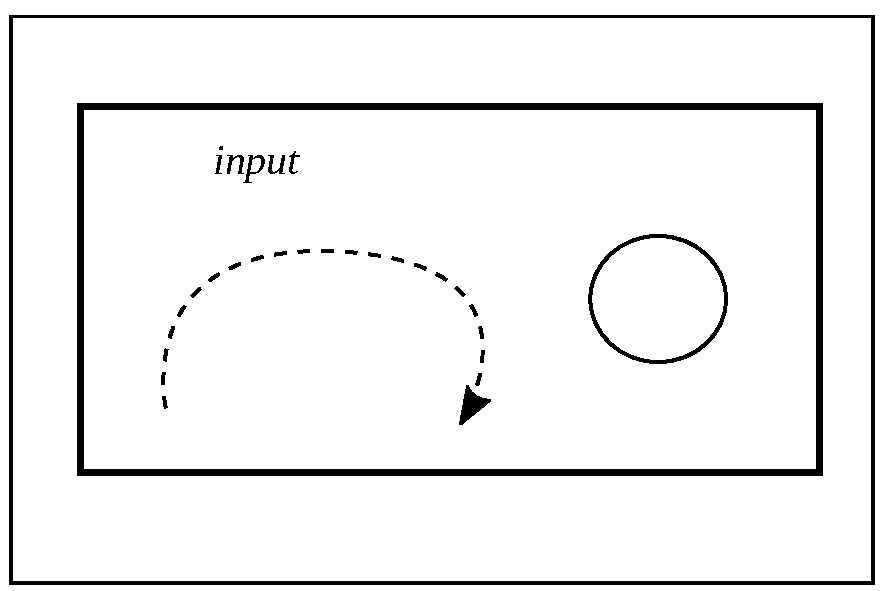
\includegraphics{images/test.pdf}}
\caption{Testuojam pdf įtraukimą.}
\end{figure}
